\documentclass[twoside]{book}

% Packages required by doxygen
\usepackage{fixltx2e}
\usepackage{calc}
\usepackage{doxygen}
\usepackage[export]{adjustbox} % also loads graphicx
\usepackage{graphicx}
\usepackage[utf8]{inputenc}
\usepackage{makeidx}
\usepackage{multicol}
\usepackage{multirow}
\PassOptionsToPackage{warn}{textcomp}
\usepackage{textcomp}
\usepackage[nointegrals]{wasysym}
\usepackage[table]{xcolor}

% Font selection
\usepackage[T1]{fontenc}
\usepackage[scaled=.90]{helvet}
\usepackage{courier}
\usepackage{amssymb}
\usepackage{sectsty}
\renewcommand{\familydefault}{\sfdefault}
\allsectionsfont{%
  \fontseries{bc}\selectfont%
  \color{darkgray}%
}
\renewcommand{\DoxyLabelFont}{%
  \fontseries{bc}\selectfont%
  \color{darkgray}%
}
\newcommand{\+}{\discretionary{\mbox{\scriptsize$\hookleftarrow$}}{}{}}

% Page & text layout
\usepackage{geometry}
\geometry{%
  a4paper,%
  top=2.5cm,%
  bottom=2.5cm,%
  left=2.5cm,%
  right=2.5cm%
}
\tolerance=750
\hfuzz=15pt
\hbadness=750
\setlength{\emergencystretch}{15pt}
\setlength{\parindent}{0cm}
\setlength{\parskip}{3ex plus 2ex minus 2ex}
\makeatletter
\renewcommand{\paragraph}{%
  \@startsection{paragraph}{4}{0ex}{-1.0ex}{1.0ex}{%
    \normalfont\normalsize\bfseries\SS@parafont%
  }%
}
\renewcommand{\subparagraph}{%
  \@startsection{subparagraph}{5}{0ex}{-1.0ex}{1.0ex}{%
    \normalfont\normalsize\bfseries\SS@subparafont%
  }%
}
\makeatother

% Headers & footers
\usepackage{fancyhdr}
\pagestyle{fancyplain}
\fancyhead[LE]{\fancyplain{}{\bfseries\thepage}}
\fancyhead[CE]{\fancyplain{}{}}
\fancyhead[RE]{\fancyplain{}{\bfseries\leftmark}}
\fancyhead[LO]{\fancyplain{}{\bfseries\rightmark}}
\fancyhead[CO]{\fancyplain{}{}}
\fancyhead[RO]{\fancyplain{}{\bfseries\thepage}}
\fancyfoot[LE]{\fancyplain{}{}}
\fancyfoot[CE]{\fancyplain{}{}}
\fancyfoot[RE]{\fancyplain{}{\bfseries\scriptsize Generated by Doxygen }}
\fancyfoot[LO]{\fancyplain{}{\bfseries\scriptsize Generated by Doxygen }}
\fancyfoot[CO]{\fancyplain{}{}}
\fancyfoot[RO]{\fancyplain{}{}}
\renewcommand{\footrulewidth}{0.4pt}
\renewcommand{\chaptermark}[1]{%
  \markboth{#1}{}%
}
\renewcommand{\sectionmark}[1]{%
  \markright{\thesection\ #1}%
}

% Indices & bibliography
\usepackage{natbib}
\usepackage[titles]{tocloft}
\setcounter{tocdepth}{3}
\setcounter{secnumdepth}{5}
\makeindex

% Hyperlinks (required, but should be loaded last)
\usepackage{ifpdf}
\ifpdf
  \usepackage[pdftex,pagebackref=true]{hyperref}
\else
  \usepackage[ps2pdf,pagebackref=true]{hyperref}
\fi
\hypersetup{%
  colorlinks=true,%
  linkcolor=blue,%
  citecolor=blue,%
  unicode%
}

% Custom commands
\newcommand{\clearemptydoublepage}{%
  \newpage{\pagestyle{empty}\cleardoublepage}%
}

\usepackage{caption}
\captionsetup{labelsep=space,justification=centering,font={bf},singlelinecheck=off,skip=4pt,position=top}

%===== C O N T E N T S =====

\begin{document}

% Titlepage & ToC
\hypersetup{pageanchor=false,
             bookmarksnumbered=true,
             pdfencoding=unicode
            }
\pagenumbering{alph}
\begin{titlepage}
\vspace*{7cm}
\begin{center}%
{\Large Spike }\\
\vspace*{1cm}
{\large Generated by Doxygen 1.8.13}\\
\end{center}
\end{titlepage}
\clearemptydoublepage
\pagenumbering{roman}
\tableofcontents
\clearemptydoublepage
\pagenumbering{arabic}
\hypersetup{pageanchor=true}

%--- Begin generated contents ---
\chapter{Hierarchical Index}
\section{Class Hierarchy}
This inheritance list is sorted roughly, but not completely, alphabetically\+:\begin{DoxyCompactList}
\item \contentsline{section}{IF}{\pageref{classIF}}{}
\begin{DoxyCompactList}
\item \contentsline{section}{L\+IF}{\pageref{classLIF}}{}
\end{DoxyCompactList}
\end{DoxyCompactList}

\chapter{Class Index}
\doxysection{Class List}
Here are the classes, structs, unions and interfaces with brief descriptions\+:\begin{DoxyCompactList}
\item\contentsline{section}{\mbox{\hyperlink{classCosineSignal}{Cosine\+Signal}} \\*Implements a cosine get\+\_\+value, i.\+e. alpha$\ast$cos(2$\ast$pi$\ast$f$\ast$t) }{\pageref{classCosineSignal}}{}
\item\contentsline{section}{\mbox{\hyperlink{classFiringRate}{Firing\+Rate}} \\*Abstract base class for firing rates. This is an abstract class that calculates the firing rate from given spike trains. One can add a spike train to a firing rate with the method add\+\_\+spike\+\_\+train, which will do the following\+: (i) it will increase the N\+\_\+neurons counter, which counts how many spike trains have been added overall and (ii) it will increase the number of spikes in the spikes histogram, which counts the spikes at a given time (these are of course determined by the time frame). One can calculate the firing rate by calling firing\+\_\+rate.\+calculate(). This of course depends on how one actually calculates the firing rate from given spike trains, which is implemented in the subclasses }{\pageref{classFiringRate}}{}
\item\contentsline{section}{\mbox{\hyperlink{classFiringRateBox}{Firing\+Rate\+Box}} \\*Implements a box firing rate. The box firing rate is calculated by counting the number of neuron that have spiked in a certain time interval (here given by the time step dt of the time frame) and dividing that number by N$\ast$dt, where N is the number of neurons overall }{\pageref{classFiringRateBox}}{}
\item\contentsline{section}{\mbox{\hyperlink{classFiringRateExp}{Firing\+Rate\+Exp}} \\*Implements an exponential firing rate. The exponential firing rate is calculated by convolving the spike train with a gaussian window function. See \cite{dayan05} }{\pageref{classFiringRateExp}}{}
\item\contentsline{section}{\mbox{\hyperlink{classFiringRateFactory}{Firing\+Rate\+Factory}} }{\pageref{classFiringRateFactory}}{}
\item\contentsline{section}{\mbox{\hyperlink{classFiringRateSimulation}{Firing\+Rate\+Simulation}} }{\pageref{classFiringRateSimulation}}{}
\item\contentsline{section}{\mbox{\hyperlink{classIF}{IF}} \\*An abstract base class for integrate-\/and-\/fire neurons }{\pageref{classIF}}{}
\item\contentsline{section}{\mbox{\hyperlink{classIFAC}{I\+F\+AC}} \\*An abstract base class for integrate-\/and-\/fire neurons with an adaptation current }{\pageref{classIFAC}}{}
\item\contentsline{section}{\mbox{\hyperlink{classLIF}{L\+IF}} \\*Implements a leaky integrate-\/and-\/fire (\mbox{\hyperlink{classLIF}{L\+IF}}) neuron }{\pageref{classLIF}}{}
\item\contentsline{section}{\mbox{\hyperlink{classLIFAC}{L\+I\+F\+AC}} \\*Implements a leaky integrate-\/and-\/fire (\mbox{\hyperlink{classLIFAC}{L\+I\+F\+AC}}) neuron }{\pageref{classLIFAC}}{}
\item\contentsline{section}{\mbox{\hyperlink{classNeuron}{Neuron}} }{\pageref{classNeuron}}{}
\item\contentsline{section}{\mbox{\hyperlink{classNeuronFactory}{Neuron\+Factory}} }{\pageref{classNeuronFactory}}{}
\item\contentsline{section}{\mbox{\hyperlink{classOptions}{Options}} \\*Implements a class that handles command line options }{\pageref{classOptions}}{}
\item\contentsline{section}{\mbox{\hyperlink{classPIF}{P\+IF}} \\*Implement a perfect integrate-\/and-\/fire (\mbox{\hyperlink{classPIF}{P\+IF}}) neuron }{\pageref{classPIF}}{}
\item\contentsline{section}{\mbox{\hyperlink{classPIFAC}{P\+I\+F\+AC}} \\*Implement a perfect integrate-\/and-\/fire (\mbox{\hyperlink{classPIFAC}{P\+I\+F\+AC}}) neuron }{\pageref{classPIFAC}}{}
\item\contentsline{section}{\mbox{\hyperlink{classSignal}{Signal}} \\*An abstract base class for signals }{\pageref{classSignal}}{}
\item\contentsline{section}{\mbox{\hyperlink{classSignalFactory}{Signal\+Factory}} \\*Implements the factory design pattern for \mbox{\hyperlink{classSignal}{Signal}} }{\pageref{classSignalFactory}}{}
\item\contentsline{section}{\mbox{\hyperlink{classSimulation}{Simulation}} }{\pageref{classSimulation}}{}
\item\contentsline{section}{\mbox{\hyperlink{classSpikeTrain}{Spike\+Train}} }{\pageref{classSpikeTrain}}{}
\item\contentsline{section}{\mbox{\hyperlink{classStepSignal}{Step\+Signal}} \\*Implement a step get\+\_\+value, i.\+e. alpha$\ast$\+Theta(t -\/ t\+\_\+0) }{\pageref{classStepSignal}}{}
\item\contentsline{section}{\mbox{\hyperlink{classTimeFrame}{Time\+Frame}} \\*A time frame class }{\pageref{classTimeFrame}}{}
\item\contentsline{section}{\mbox{\hyperlink{classTwoCosineSignal}{Two\+Cosine\+Signal}} \\*Implements a get\+\_\+value consisting of two cosine, i.\+e. alpha$\ast$cos(2$\ast$pi$\ast$f1$\ast$t) }{\pageref{classTwoCosineSignal}}{}
\item\contentsline{section}{\mbox{\hyperlink{classWhiteNoiseSignal}{White\+Noise\+Signal}} \\*Implements a band limited white gaussian noise get\+\_\+value }{\pageref{classWhiteNoiseSignal}}{}
\end{DoxyCompactList}

\chapter{Class Documentation}
\hypertarget{classIF}{}\section{IF Class Reference}
\label{classIF}\index{IF@{IF}}


{\ttfamily \#include $<$models.\+h$>$}



Inheritance diagram for IF\+:\nopagebreak
\begin{figure}[H]
\begin{center}
\leavevmode
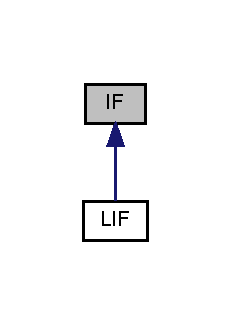
\includegraphics[width=111pt]{classIF__inherit__graph}
\end{center}
\end{figure}
\subsection*{Public Member Functions}
\begin{DoxyCompactItemize}
\item 
virtual double \hyperlink{classIF_a9bbd53df68cb9028bf87cf5273253e91}{drift} (double v, double t)
\item 
\mbox{\Hypertarget{classIF_a45c14ff90b19a93769c2c30741cd482d}\label{classIF_a45c14ff90b19a93769c2c30741cd482d}} 
virtual double {\bfseries diffusion} (double v, double t)
\end{DoxyCompactItemize}
\subsection*{Public Attributes}
\begin{DoxyCompactItemize}
\item 
int \hyperlink{classIF_aa81bddacf949214f2265214d7174f4c2}{N}
\item 
\mbox{\Hypertarget{classIF_ab9ff14c2b3690db446567d26cdf21540}\label{classIF_ab9ff14c2b3690db446567d26cdf21540}} 
double {\bfseries t\+\_\+0}
\item 
\mbox{\Hypertarget{classIF_a2c512964adfc0421306b655ba3c85d3d}\label{classIF_a2c512964adfc0421306b655ba3c85d3d}} 
double {\bfseries t\+\_\+end}
\item 
\mbox{\Hypertarget{classIF_a9f690c993d7b7cd0095e26607503db72}\label{classIF_a9f690c993d7b7cd0095e26607503db72}} 
double {\bfseries mu}
\item 
\mbox{\Hypertarget{classIF_a7e0fdbf32975dba0acf8096524885639}\label{classIF_a7e0fdbf32975dba0acf8096524885639}} 
double {\bfseries D}
\end{DoxyCompactItemize}


\subsection{Detailed Description}
Defines the integrate and fire (\hyperlink{classIF}{IF}) neuron, defaults to perfect \hyperlink{classIF}{IF} 

\subsection{Member Function Documentation}
\mbox{\Hypertarget{classIF_a9bbd53df68cb9028bf87cf5273253e91}\label{classIF_a9bbd53df68cb9028bf87cf5273253e91}} 
\index{IF@{IF}!drift@{drift}}
\index{drift@{drift}!IF@{IF}}
\subsubsection{\texorpdfstring{drift()}{drift()}}
{\footnotesize\ttfamily virtual double I\+F\+::drift (\begin{DoxyParamCaption}\item[{double}]{v,  }\item[{double}]{t }\end{DoxyParamCaption})\hspace{0.3cm}{\ttfamily [inline]}, {\ttfamily [virtual]}}

drift and diffusion functions, can be overwritten by subclasses 

Reimplemented in \hyperlink{classLIF_aea677a0cf3f943edb7a957479e18d6dc}{L\+IF}.



\subsection{Member Data Documentation}
\mbox{\Hypertarget{classIF_aa81bddacf949214f2265214d7174f4c2}\label{classIF_aa81bddacf949214f2265214d7174f4c2}} 
\index{IF@{IF}!N@{N}}
\index{N@{N}!IF@{IF}}
\subsubsection{\texorpdfstring{N}{N}}
{\footnotesize\ttfamily int I\+F\+::N}

Simulation parameters 
\begin{DoxyParams}{Parameters}
{\em N} & Number of times steps \\
\hline
{\em t\+\_\+0} & Starting time \\
\hline
{\em t\+\_\+end} & End time \\
\hline
{\em mu} & \\
\hline
{\em D} & Diffusion coefficient \\
\hline
\end{DoxyParams}


The documentation for this class was generated from the following file\+:\begin{DoxyCompactItemize}
\item 
/home/cheg/\+Repos/\+Master/\+Spike/src/models.\+h\end{DoxyCompactItemize}

\hypertarget{classLIF}{}\section{L\+IF Class Reference}
\label{classLIF}\index{L\+IF@{L\+IF}}


{\ttfamily \#include $<$models.\+h$>$}



Inheritance diagram for L\+IF\+:\nopagebreak
\begin{figure}[H]
\begin{center}
\leavevmode
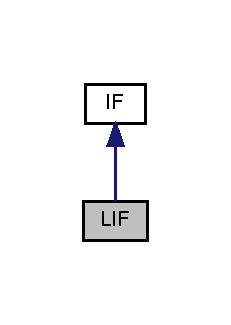
\includegraphics[width=111pt]{classLIF__inherit__graph}
\end{center}
\end{figure}


Collaboration diagram for L\+IF\+:\nopagebreak
\begin{figure}[H]
\begin{center}
\leavevmode
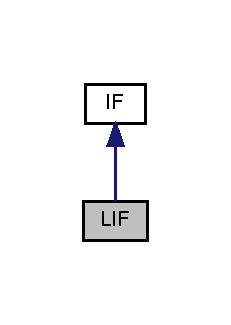
\includegraphics[width=111pt]{classLIF__coll__graph}
\end{center}
\end{figure}
\subsection*{Public Member Functions}
\begin{DoxyCompactItemize}
\item 
double \hyperlink{classLIF_aea677a0cf3f943edb7a957479e18d6dc}{drift} (double v, double t)
\end{DoxyCompactItemize}
\subsection*{Additional Inherited Members}


\subsection{Detailed Description}
Defines leaky integrate and fire neuron, inherits everything from \hyperlink{classIF}{IF} 

\subsection{Member Function Documentation}
\mbox{\Hypertarget{classLIF_aea677a0cf3f943edb7a957479e18d6dc}\label{classLIF_aea677a0cf3f943edb7a957479e18d6dc}} 
\index{L\+IF@{L\+IF}!drift@{drift}}
\index{drift@{drift}!L\+IF@{L\+IF}}
\subsubsection{\texorpdfstring{drift()}{drift()}}
{\footnotesize\ttfamily double L\+I\+F\+::drift (\begin{DoxyParamCaption}\item[{double}]{v,  }\item[{double}]{t }\end{DoxyParamCaption})\hspace{0.3cm}{\ttfamily [inline]}, {\ttfamily [virtual]}}

change the drift 

Reimplemented from \hyperlink{classIF_a9bbd53df68cb9028bf87cf5273253e91}{IF}.



The documentation for this class was generated from the following file\+:\begin{DoxyCompactItemize}
\item 
/home/cheg/\+Repos/\+Master/\+Spike/src/\+Models/models.\+h\end{DoxyCompactItemize}

%--- End generated contents ---

% Index
\backmatter
\newpage
\phantomsection
\clearemptydoublepage
\addcontentsline{toc}{chapter}{Index}
\printindex

\end{document}
